% METODOLOGIA------------------------------------------------------------------

\chapter{PARADIGMA}
\label{chap:paradigma}

\section{CONSTRUÇÕES}
\label{sec:construcoes}

Construções de Python incluem: estrutura de seleção \textit{(if, else, elif)};
estrutura de repetição \textit{(for, while)}, que itera por um container, capturando cada elemento em uma variável local dada;
construção de classes (class); construção de sub-rotinas \textit{(def)};
construção de escopo \textit{(with)}, como por exemplo para adquirir um recurso.

\begin{figure}[!htb]
    \centering
    \caption{Python 3 The Standard type hyerarchy}
    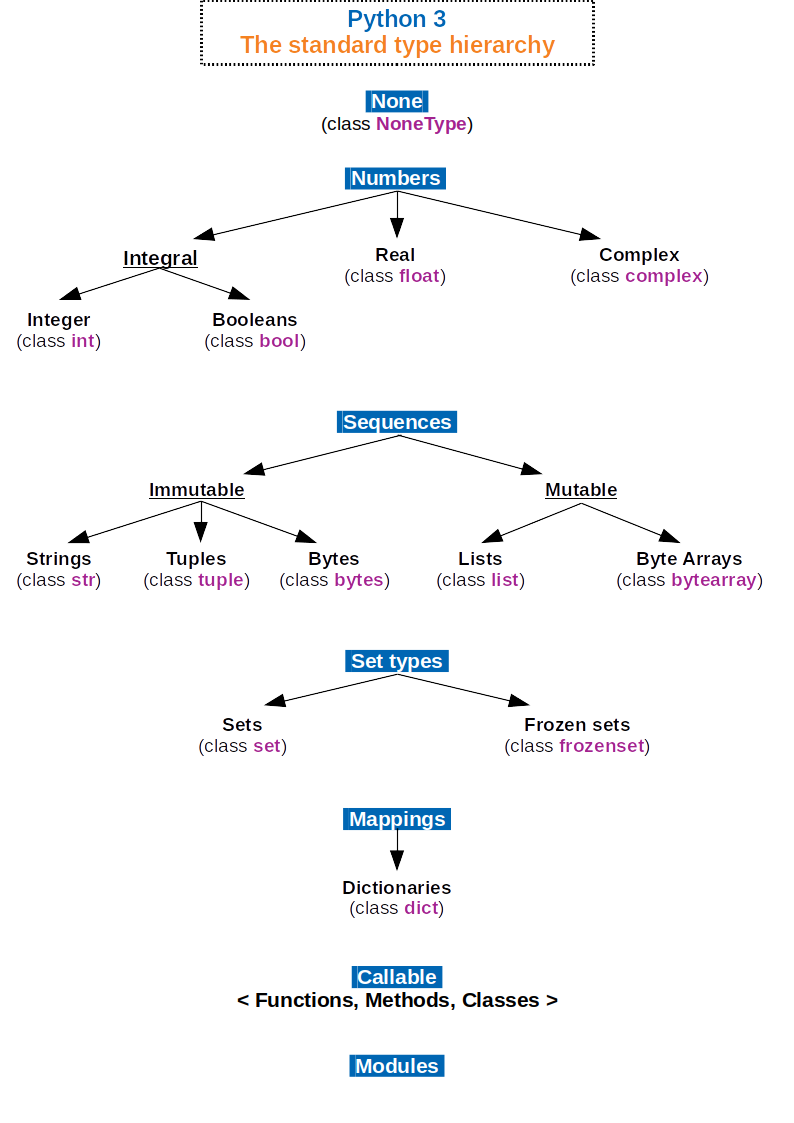
\includegraphics[width=0.75\textwidth]{./dados/figuras/Python_3._The_standard_type_hierarchy.png}
    \fonte{\url{https://pt.wikipedia.org/wiki/Ficheiro:Python_3._The_standard_type_hierarchy.png}}
    \label{fig:figura-tipos-python}
\end{figure}

\section{TIPOS DE DADOS}
\label{sec:tiposDados}

A tipagem de Python é forte, pois os valores e objetos têm tipos bem definidos e não sofrem coerções como em C ou Perl.
São disponibilizados diversos tipos de dados nativos:\footnote{
    O tipo int (inteiro) é transparentemente convertido para long caso não caiba em um int.
}
\footnote{
    Os Tipos set e frozenset não contém elementos duplicados
}

\begin{table}[!htb]
    \centering
    \caption[Tipos de dados em Python]{Tipos de dados em Python.
    \label{tab:tipos-dados}}
    \begin{tabular}{rrrrr}
        \toprule
        Tipo de dados & Descrição & Exemplo de sintaxe \\
        \midrule
        str, unicode    & Uma cadeia de caracteres imutável & 'foo'; "bar"  \\
        list    & Lista heterogênea mutável & [4.0, 'string', True]  \\
        tuple    & Tupla imutável & (4.0, 'string', True)  \\
        set, frozenset    & Conjunto não ordenado & set([4.0, 'string', True])  \\
        dict    & conjunto associativo & \{'key1': 1.0, 'key2': False\}  \\
        int    & Número de precisão fixa & 42; 2147483648L \\
        float    & Ponto flutuante & 3.1415927  \\
        complex    & Número complexo & $3+2j$  \\
        bool    & Booleano & True; False  \\
        $!=$    & Diferente & Diferente  \\
        \bottomrule
    \end{tabular}
    \fonte{\citeonline{PyDoc}}
\end{table}

Python também permite a definição dos tipos de dados próprios, através de classes.
Instâncias são construídas invocando a classe \textit{(FooClass())}, e as classes são instância da classe type, o que permite metaprogramação e reflexão.
Métodos são definidos como funções anexadas à classe, e a sintaxe \textit{instância.método(argumento)} é um atalho para \textit{Classe.método(instância, argumento)}.
Os métodos devem referenciar explicitamente a referência para o objeto incluindo o parâmetro self como o primeiro argumento do método.
Antes da versão 3.0, Python possuía dois tipos de classes: "old-style" e "new-style". Classes old-style foram eliminadas no Python 3.0, e todas são new-style. Em versões entre 2.2 e 3.0, ambos tipos de classes podiam ser usadas. A sintaxe de ambos estilos é a mesma, a diferença acaba sendo de onde objeto da classe é herdado, direta ou indiretamente (todas classes new-style herdam de objeto e são instâncias de type).
As classes new-styles nada mais são que tipos definidos pelo usuário.

\section{PALAVRAS RESERVADAS}
O Python 3 define as seguintes palavras reservadas:
\begin{itemize}
    \item \textbf{False}
    \item \textbf{None}
    \item \textbf{True}
    \item \textbf{and}
    \item \textbf{as}
    \item \textbf{assert}
    \item \textbf{break}
    \item \textbf{class}
    \item \textbf{continue}
    \item \textbf{def}
    \item \textbf{del}
    \item \textbf{elif}
    \item \textbf{else}
    \item \textbf{except}
    \item \textbf{finally}
    \item \textbf{for}
    \item \textbf{from}
    \item \textbf{global}
    \item \textbf{if}
    \item \textbf{import}
    \item \textbf{in}
    \item \textbf{is}
    \item \textbf{lambda}
    \item \textbf{not}
    \item \textbf{nonlocal}
    \item \textbf{or}
    \item \textbf{pass}
    \item \textbf{raise}
    \item \textbf{try}
    \item \textbf{return}
    \item \textbf{while}
    \item \textbf{with}
    \item \textbf{yield}
\end{itemize}

\section{OPERADORES}
Os operadores básicos de comparação como $==$, $<$, $>=$, entre outros são usados em todos os tipos de dados, como números, cadeias de texto, listas e mapeamentos.
Comparações em cadeia como $a < b < c$ possuem o mesmo significado básico que na matemática: os termos são comparadas na ordem.
É garantido que o processamento da expressão lógica irá terminar tão cedo o veredito seja claro, o princípio da avaliação mínima.
Usando a expressão anterior, se $a < b$ é falso, $c$ não é avaliado.
\par Quanto aos operadores lógicos, até Python 2.2 não havia o tipo de dado booleano.
Em todas as versões da linguagem os operadores lógicos\footnote{
    Na versão 2.2.1 as constantes True e False foram adicionadas (subclasses de 1 e 0 respectivamente)
} tratam \textit{"", 0, None, 0.0, [] e {}} como falso, enquanto o restante é tratado como verdadeiro de modo geral.
A comparação binária retorna uma das duas constantes acima.
\par Os operadores booleanos and e or também seguem a avaliação mínima. Por exemplo, $y == 0 or x/y > 100$ nunca lançará a exceção de divisão por zero.

\section{INTERPRETADOR INTERATIVO}
O interpretador interativo é uma característica diferencial da linguagem, porque há a possibilidade de testar o código de um programa e receber o resultado em tempo real, antes de iniciar a compilação ou incluí-las nos programas. 
Por exemplo:\footnote{
    A partir da versão 3.0, o comando print passou a ser uma função, sendo obrigatório o uso de parênteses.
}\\
\begin{algorithm}
    \caption{Exemplo do Interpretador Interativo}
    $>>>$ 1+1\\
    2\\
    $>>>$\\
    $>>>$ a = 1+1\\
    $>>>$ \textbf{print} a\\
    2\\
    $>>>$ \textbf{print}(a)\\
    2\\
    $>>>$\\
\end{algorithm}



